\documentclass[12pt,a4paper]{article}
\usepackage[utf8]{inputenc}
\usepackage[english]{babel}
\usepackage{geometry}
\usepackage{fancyhdr}
\usepackage{graphicx}
\usepackage{float}
\usepackage{tabularx}
\usepackage{longtable}
\usepackage{array}
\usepackage{booktabs}
\usepackage{multirow}
\usepackage{listings}
\usepackage{xcolor}
\usepackage{hyperref}
\usepackage{amsmath}
\usepackage{amsfonts}
\usepackage{amssymb}
\usepackage{enumitem}
\usepackage{caption}
\usepackage{subcaption}

% Page setup
\geometry{
    left=2.5cm,
    right=2.5cm,
    top=2.5cm,
    bottom=2.5cm
}

% Header and footer
\pagestyle{fancy}
\fancyhf{}
\rhead{HIV Clinic Management System}
\lhead{Software Design Specification}
\cfoot{\thepage}

% Code listing style
\lstset{
    basicstyle=\ttfamily\small,
    breaklines=true,
    frame=single,
    language=Java,
    numbers=left,
    numberstyle=\tiny,
    showstringspaces=false,
    tabsize=2,
    commentstyle=\color{gray},
    keywordstyle=\color{blue},
    stringstyle=\color{red}
}

% Define colors
\definecolor{packagecolor}{RGB}{173, 216, 230}
\definecolor{classcolor}{RGB}{255, 218, 185}
\definecolor{interfacecolor}{RGB}{221, 160, 221}

% Title page
\title{
    \vspace{-2cm}
    \Huge\textbf{HIV Clinic Management System}\\
    \vspace{1cm}
    \Large\textbf{Software Design Specification}\\
    \vspace{2cm}
    \normalsize Version 2.0
}

\author{}
\date{
    \vspace{4cm}
    – Ho Chi Minh City, January 2025 –
}

\begin{document}

\maketitle
\thispagestyle{empty}

\newpage

% Record of changes
\section*{Record of Changes}
\begin{longtable}{|p{3cm}|p{2cm}|p{3cm}|p{6cm}|}
\hline
\textbf{Date} & \textbf{A*M, D} & \textbf{In charge} & \textbf{Change Description} \\
\hline
2025-01-08 & A & System Architect & Complete regeneration based on current codebase \\
\hline
2025-01-08 & A & System Architect & Updated architecture to reflect Spring Boot 3.2.0 \\
\hline
2025-01-08 & A & System Architect & Enhanced domain model documentation \\
\hline
2025-01-08 & A & System Architect & Updated API specifications and security model \\
\hline
\end{longtable}

\textit{*A - Added M - Modified D - Deleted}

\newpage

\tableofcontents

\newpage

\section{Introduction}

\subsection{Purpose}
This Software Design Specification (SDS) document provides a comprehensive technical design overview of the HIV Clinic Management System. It defines the system architecture, component design, data models, and implementation details based on the current Spring Boot 3.2.0 and React 18.2.0 implementation.

\subsection{Scope}
The HIV Clinic Management System is a web-based application designed to manage HIV clinic operations including:
\begin{itemize}
    \item Patient registration and profile management with privacy controls
    \item Multi-role authentication and authorization (Guest, Patient, Doctor, Admin, Manager)
    \item Comprehensive appointment scheduling with doctor availability management
    \item ARV (Antiretroviral) treatment tracking and medication routine management
    \item Advanced notification system with template-based messaging
    \item Patient record management with audit trail
    \item Administrative functions and system monitoring
\end{itemize}

\subsection{System Overview}
The system implements a modern three-tier architecture:
\begin{itemize}
    \item \textbf{Presentation Layer}: React 18.2.0 single-page application with Vite build system
    \item \textbf{Business Logic Layer}: Spring Boot 3.2.0 RESTful web services with Java 17
    \item \textbf{Data Layer}: Microsoft SQL Server with Hibernate JPA and connection pooling
\end{itemize}

\section{System Architecture}

\subsection{High-Level Architecture}

\begin{figure}[H]
\centering
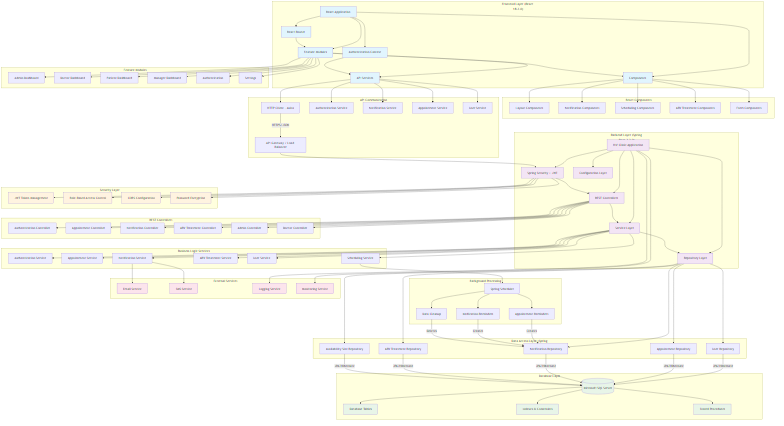
\includegraphics[width=0.9\textwidth]{diagrams/system_architecture}
\caption{System Architecture Overview}
\label{fig:system-architecture}
\end{figure}

The system follows a microservice-oriented monolithic architecture with clear separation of concerns:

\subsubsection{Frontend Layer (React 18.2.0)}
\begin{itemize}
    \item \textbf{React Router DOM 6.8.0}: Client-side routing with role-based route protection
    \item \textbf{Context API}: Global state management for authentication and user context
    \item \textbf{Axios}: HTTP client for API communication with interceptors for JWT handling
    \item \textbf{Vite}: Fast build tool with hot module replacement for development
    \item \textbf{Component Architecture}: Feature-based organization with reusable UI components
\end{itemize}

\subsubsection{Backend Layer (Spring Boot 3.2.0)}
\begin{itemize}
    \item \textbf{Spring Security}: JWT-based authentication with role-based authorization
    \item \textbf{Spring Data JPA}: Repository pattern with Hibernate as ORM
    \item \textbf{Spring Web MVC}: RESTful API controllers with comprehensive error handling
    \item \textbf{Spring Validation}: Bean validation with custom validators
    \item \textbf{Spring Scheduling}: Automated tasks for notifications and system maintenance
\end{itemize}

\subsubsection{Data Layer}
\begin{itemize}
    \item \textbf{Microsoft SQL Server}: Primary database with ACID compliance
    \item \textbf{HikariCP}: High-performance connection pool with configuration optimization
    \item \textbf{Database Migrations}: Schema versioning through Hibernate DDL auto-update
\end{itemize}

\subsection{Component Architecture}

\begin{figure}[H]
\centering
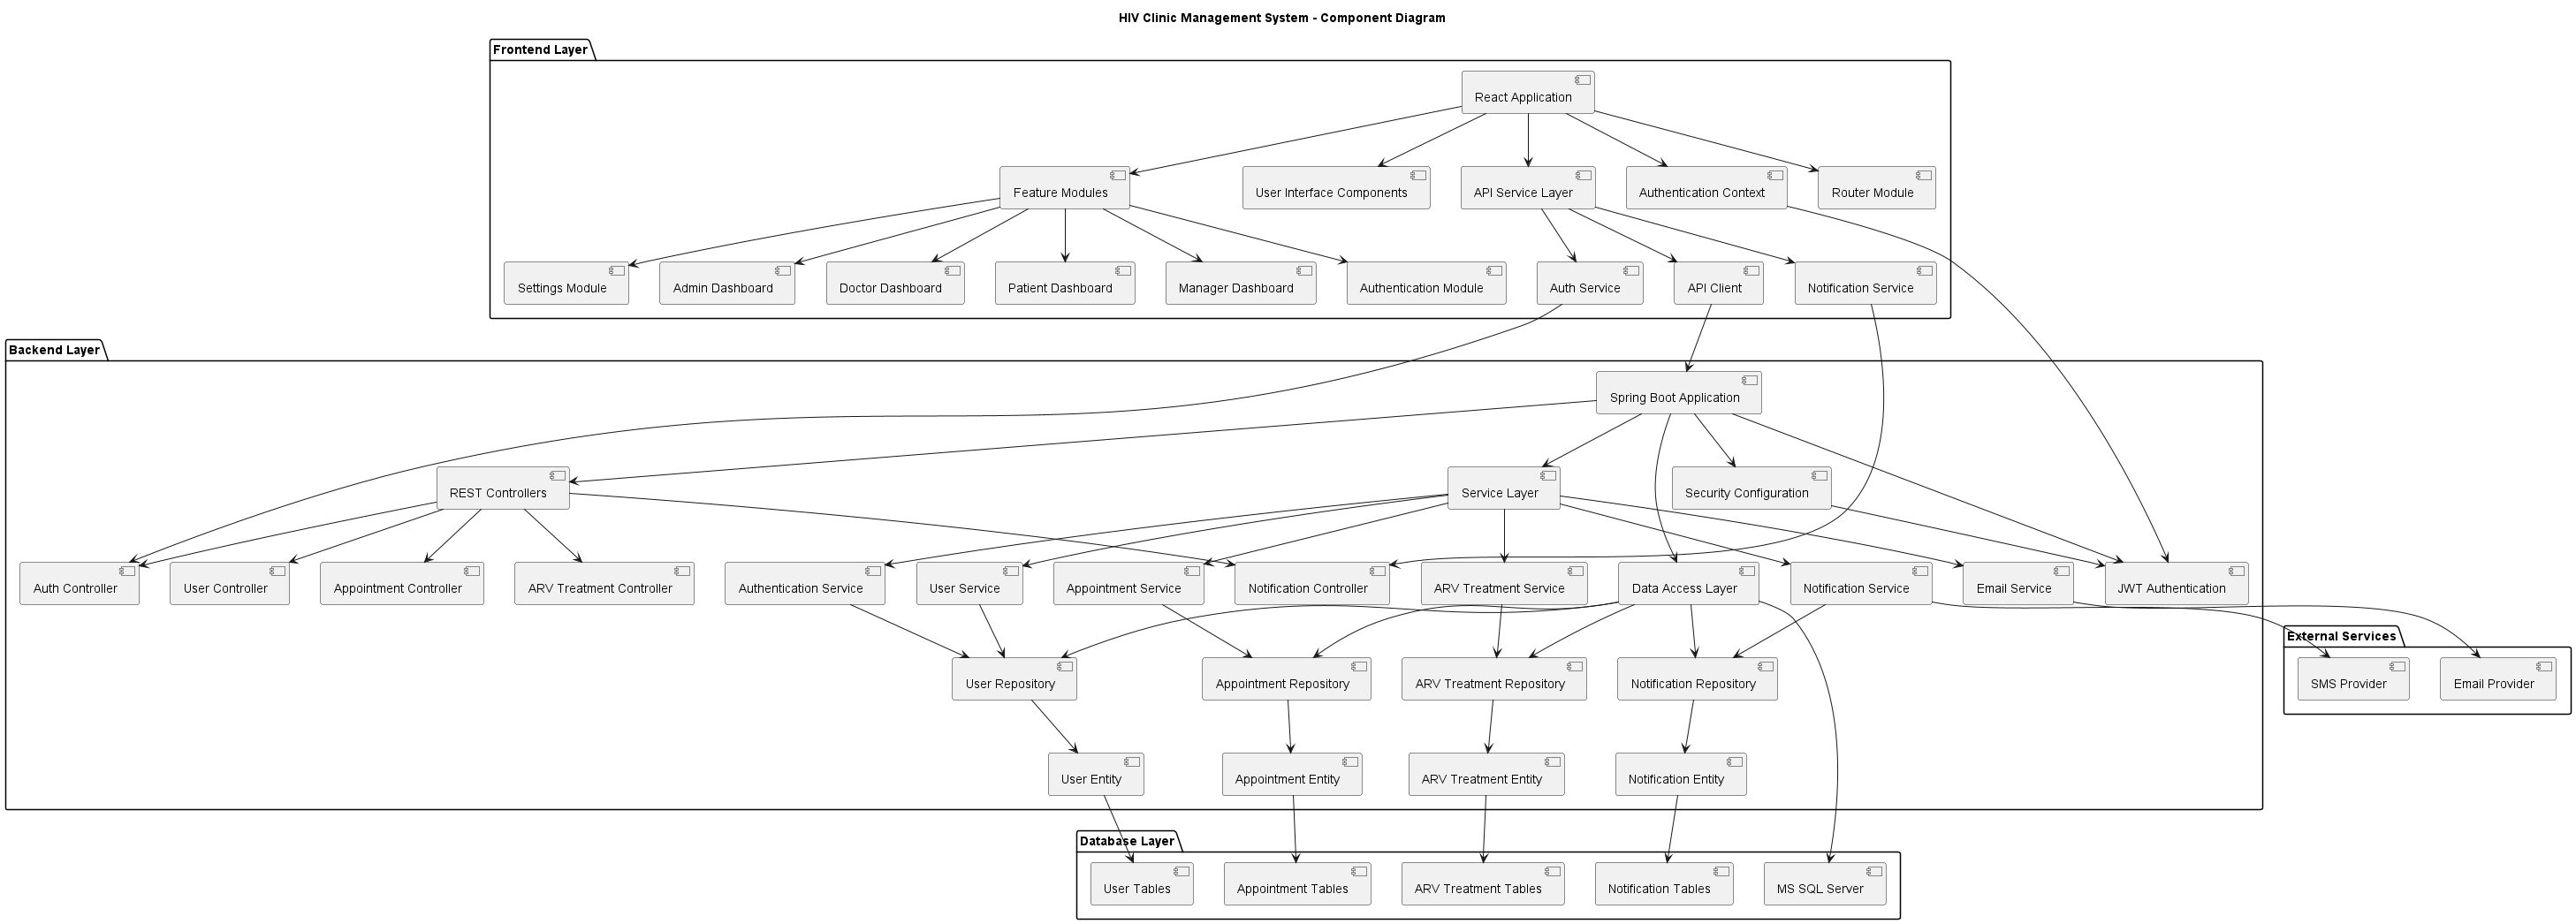
\includegraphics[width=0.9\textwidth]{diagrams/component_diagram}
\caption{Component Diagram}
\label{fig:component-diagram}
\end{figure}

\subsubsection{Backend Components}

\paragraph{Controller Layer}
The controller layer implements RESTful endpoints with comprehensive CRUD operations:

\begin{longtable}{|p{3cm}|p{4cm}|p{7cm}|}
\hline
\textbf{Controller} & \textbf{Base Path} & \textbf{Responsibilities} \\
\hline
AuthController & /api/auth & User registration, login, logout, password management \\
\hline
AppointmentController & /api/appointments & Appointment CRUD, scheduling, status management \\
\hline
PatientRecordController & /api/patient-records & Medical record management, history tracking \\
\hline
ARVTreatmentController & /api/arv-treatments & ARV treatment plans, medication tracking \\
\hline
NotificationController & /api/notifications & Notification delivery, template management \\
\hline
AdminController & /api/admin & User management, system administration \\
\hline
DoctorController & /api/doctors & Doctor profile, availability management \\
\hline
ManagerController & /api/manager & Reporting, analytics, resource management \\
\hline
\end{longtable}

\paragraph{Service Layer}
Business logic implementation with transaction management:

\begin{longtable}{|p{3cm}|p{9cm}|}
\hline
\textbf{Service} & \textbf{Core Responsibilities} \\
\hline
AuthService & JWT token generation, user authentication, password encryption \\
\hline
AppointmentService & Appointment scheduling logic, conflict resolution, status workflows \\
\hline
ARVTreatmentService & Treatment plan creation, medication routine management \\
\hline
NotificationService & Message delivery, template processing, scheduling \\
\hline
PatientRecordService & Medical record management, privacy enforcement \\
\hline
DoctorAvailabilityService & Doctor schedule management, slot allocation \\
\hline
UserSessionService & Session tracking, concurrent login management \\
\hline
\end{longtable}

\paragraph{Repository Layer}
Data access with Spring Data JPA repositories:

\begin{longtable}{|p{3cm}|p{9cm}|}
\hline
\textbf{Repository} & \textbf{Custom Query Methods} \\
\hline
UserRepository & findByUsername, findByEmail, findByRoleAndIsActive \\
\hline
AppointmentRepository & findByPatientAndDateRange, findByDoctorAndStatus \\
\hline
PatientRecordRepository & findByPatientUserID, findByAppointmentId \\
\hline
NotificationRepository & findByUserAndStatus, findByTypeAndScheduledTime \\
\hline
ARVTreatmentRepository & findByPatientAndIsActive, findByMedicationName \\
\hline
\end{longtable}

\subsubsection{Frontend Components}

\paragraph{Feature Modules}
Role-based feature organization:

\begin{longtable}{|p{3cm}|p{9cm}|}
\hline
\textbf{Feature Module} & \textbf{Components} \\
\hline
Admin & UserManagement, SystemSettings, AuditLogs, Analytics \\
\hline
Doctor & AppointmentCalendar, PatientRecords, AvailabilityManager \\
\hline
Patient & AppointmentBooking, MedicalHistory, TreatmentPlan \\
\hline
Manager & ReportsDashboard, ResourceManagement, StaffScheduling \\
\hline
Auth & LoginForm, RegisterForm, PasswordReset, UserProfile \\
\hline
\end{longtable}

\paragraph{Shared Components}
Reusable UI components:

\begin{longtable}{|p{3cm}|p{9cm}|}
\hline
\textbf{Component Category} & \textbf{Components} \\
\hline
Layout & Header, Sidebar, Footer, NavigationMenu \\
\hline
UI & Button, Input, Modal, Table, Calendar, Charts \\
\hline
Notifications & ToastNotification, NotificationCenter, AlertBanner \\
\hline
Forms & FormField, Validation, FileUpload, DatePicker \\
\hline
\end{longtable}

\section{Database Design}

\subsection{Entity Relationship Diagram}

\begin{figure}[H]
\centering
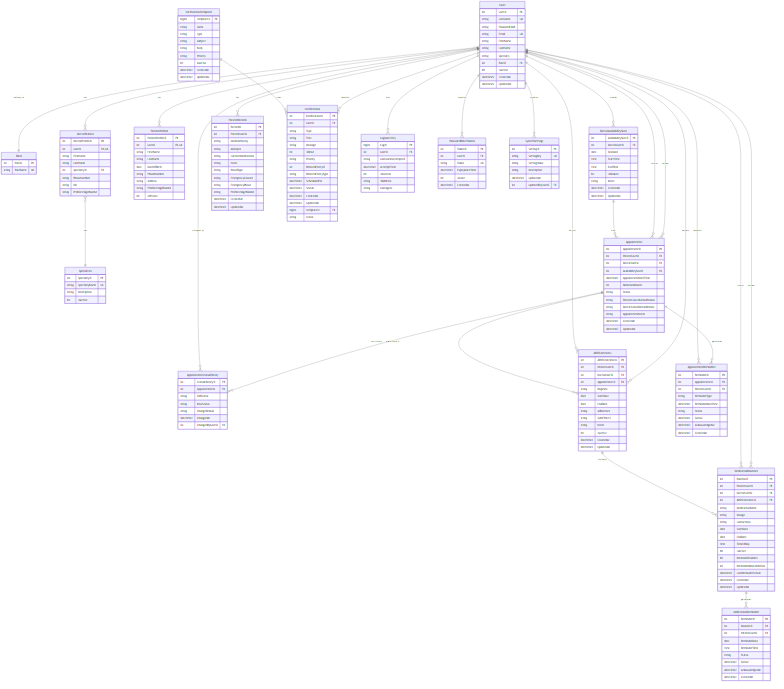
\includegraphics[width=0.9\textwidth]{diagrams/database_schema_erd}
\caption{Database Schema ERD}
\label{fig:database-erd}
\end{figure}

\subsection{Core Entities}

\subsubsection{User Management}

\paragraph{Users Entity}
Central user table with role-based access control:

\begin{lstlisting}[language=SQL]
CREATE TABLE Users (
    UserID int IDENTITY(1,1) PRIMARY KEY,
    Username nvarchar(50) UNIQUE NOT NULL,
    PasswordHash nvarchar(255) NOT NULL,
    Email nvarchar(100) UNIQUE NOT NULL,
    FirstName nvarchar(50),
    LastName nvarchar(50),
    Specialty nvarchar(100),
    RoleID int FOREIGN KEY REFERENCES Roles(RoleID),
    IsActive bit DEFAULT 1,
    CreatedAt datetime2 DEFAULT GETDATE(),
    UpdatedAt datetime2 DEFAULT GETDATE()
);
\end{lstlisting}

\paragraph{Roles Entity}
Role definition for authorization:

\begin{lstlisting}[language=SQL]
CREATE TABLE Roles (
    RoleID int IDENTITY(1,1) PRIMARY KEY,
    RoleName nvarchar(50) UNIQUE NOT NULL
);

-- Initial roles
INSERT INTO Roles (RoleName) VALUES 
('ADMIN'), ('DOCTOR'), ('PATIENT'), ('MANAGER'), ('GUEST');
\end{lstlisting}

\subsubsection{Patient Management}

\paragraph{PatientProfiles Entity}
Extended patient information with privacy controls:

\begin{lstlisting}[language=SQL]
CREATE TABLE PatientProfiles (
    PatientProfileID int IDENTITY(1,1) PRIMARY KEY,
    UserID int FOREIGN KEY REFERENCES Users(UserID),
    FirstName nvarchar(50),
    LastName nvarchar(50),
    DateOfBirth date,
    PhoneNumber nvarchar(20),
    Address nvarchar(255),
    ProfileImageBase64 nvarchar(MAX),
    IsPrivate bit DEFAULT 0
);
\end{lstlisting}

\paragraph{PatientRecords Entity}
Medical records with comprehensive tracking:

\begin{lstlisting}[language=SQL]
CREATE TABLE PatientRecords (
    RecordID int IDENTITY(1,1) PRIMARY KEY,
    PatientUserID int FOREIGN KEY REFERENCES Users(UserID),
    AppointmentId int FOREIGN KEY REFERENCES Appointments(AppointmentID),
    MedicalHistory nvarchar(MAX),
    Allergies nvarchar(MAX),
    CurrentMedications nvarchar(MAX),
    Notes nvarchar(MAX),
    BloodType nvarchar(10),
    EmergencyContact nvarchar(100),
    EmergencyPhone nvarchar(20),
    CreatedAt datetime2 DEFAULT GETDATE(),
    UpdatedAt datetime2 DEFAULT GETDATE()
);
\end{lstlisting}

\subsubsection{Appointment System}

\paragraph{Appointments Entity}
Core appointment management with status tracking:

\begin{lstlisting}[language=SQL]
CREATE TABLE Appointments (
    AppointmentID int IDENTITY(1,1) PRIMARY KEY,
    PatientUserID int FOREIGN KEY REFERENCES Users(UserID),
    DoctorUserID int FOREIGN KEY REFERENCES Users(UserID),
    AvailabilitySlotID int FOREIGN KEY REFERENCES DoctorAvailabilitySlots(SlotID),
    AppointmentDateTime datetime2 NOT NULL,
    DurationMinutes int DEFAULT 30,
    Status nvarchar(50) DEFAULT 'Scheduled',
    Notes nvarchar(MAX),
    CreatedAt datetime2 DEFAULT GETDATE(),
    UpdatedAt datetime2 DEFAULT GETDATE()
);
\end{lstlisting}

\paragraph{DoctorAvailabilitySlots Entity}
Doctor schedule management:

\begin{lstlisting}[language=SQL]
CREATE TABLE DoctorAvailabilitySlots (
    SlotID int IDENTITY(1,1) PRIMARY KEY,
    DoctorUserID int FOREIGN KEY REFERENCES Users(UserID),
    SlotDateTime datetime2 NOT NULL,
    DurationMinutes int DEFAULT 30,
    IsAvailable bit DEFAULT 1,
    MaxAppointments int DEFAULT 1,
    Notes nvarchar(255)
);
\end{lstlisting}

\subsubsection{ARV Treatment System}

\paragraph{ARVTreatments Entity}
Antiretroviral treatment tracking:

\begin{lstlisting}[language=SQL]
CREATE TABLE ARVTreatments (
    TreatmentID int IDENTITY(1,1) PRIMARY KEY,
    PatientUserID int FOREIGN KEY REFERENCES Users(UserID),
    DoctorUserID int FOREIGN KEY REFERENCES Users(UserID),
    MedicationName nvarchar(100) NOT NULL,
    Dosage nvarchar(50),
    Frequency nvarchar(50),
    StartDate date NOT NULL,
    EndDate date,
    Instructions nvarchar(MAX),
    SideEffects nvarchar(MAX),
    IsActive bit DEFAULT 1,
    CreatedAt datetime2 DEFAULT GETDATE(),
    UpdatedAt datetime2 DEFAULT GETDATE()
);
\end{lstlisting}

\paragraph{MedicationRoutines Entity}
Daily medication schedule management:

\begin{lstlisting}[language=SQL]
CREATE TABLE MedicationRoutines (
    RoutineID int IDENTITY(1,1) PRIMARY KEY,
    PatientUserID int FOREIGN KEY REFERENCES Users(UserID),
    TreatmentID int FOREIGN KEY REFERENCES ARVTreatments(TreatmentID),
    MedicationName nvarchar(100),
    DosageAmount nvarchar(50),
    ScheduledTime time,
    Frequency nvarchar(50),
    Instructions nvarchar(MAX),
    IsActive bit DEFAULT 1,
    CreatedAt datetime2 DEFAULT GETDATE()
);
\end{lstlisting}

\subsubsection{Notification System}

\paragraph{Notifications Entity}
Comprehensive notification management:

\begin{lstlisting}[language=SQL]
CREATE TABLE Notifications (
    NotificationID int IDENTITY(1,1) PRIMARY KEY,
    UserID int FOREIGN KEY REFERENCES Users(UserID),
    TemplateID int FOREIGN KEY REFERENCES NotificationTemplates(TemplateID),
    Title nvarchar(255) NOT NULL,
    Message nvarchar(MAX) NOT NULL,
    Type nvarchar(50) DEFAULT 'INFO',
    Status nvarchar(50) DEFAULT 'PENDING',
    ScheduledAt datetime2,
    SentAt datetime2,
    ReadAt datetime2,
    Priority nvarchar(20) DEFAULT 'MEDIUM',
    CreatedAt datetime2 DEFAULT GETDATE()
);
\end{lstlisting}

\paragraph{NotificationTemplates Entity}
Template-based messaging system:

\begin{lstlisting}[language=SQL]
CREATE TABLE NotificationTemplates (
    TemplateID int IDENTITY(1,1) PRIMARY KEY,
    TemplateName nvarchar(100) UNIQUE NOT NULL,
    Subject nvarchar(255),
    MessageTemplate nvarchar(MAX) NOT NULL,
    Type nvarchar(50),
    IsActive bit DEFAULT 1,
    CreatedAt datetime2 DEFAULT GETDATE(),
    UpdatedAt datetime2 DEFAULT GETDATE()
);
\end{lstlisting}

\section{API Design}

\subsection{RESTful API Endpoints}

\subsubsection{Authentication API}

\begin{longtable}{|p{1.5cm}|p{4cm}|p{6.5cm}|}
\hline
\textbf{Method} & \textbf{Endpoint} & \textbf{Description} \\
\hline
POST & /api/auth/register & User registration with role assignment \\
\hline
POST & /api/auth/login & JWT authentication with session tracking \\
\hline
POST & /api/auth/logout & Session invalidation and cleanup \\
\hline
GET & /api/auth/profile & Current user profile information \\
\hline
PUT & /api/auth/profile & Update user profile data \\
\hline
POST & /api/auth/change-password & Secure password change operation \\
\hline
POST & /api/auth/forgot-password & Password reset request initiation \\
\hline
POST & /api/auth/reset-password & Password reset with token validation \\
\hline
\end{longtable}

\subsubsection{Appointment Management API}

\begin{longtable}{|p{1.5cm}|p{4cm}|p{6.5cm}|}
\hline
\textbf{Method} & \textbf{Endpoint} & \textbf{Description} \\
\hline
GET & /api/appointments & List appointments with filtering and pagination \\
\hline
POST & /api/appointments & Create new appointment with validation \\
\hline
GET & /api/appointments/\{id\} & Retrieve specific appointment details \\
\hline
PUT & /api/appointments/\{id\} & Update appointment information \\
\hline
DELETE & /api/appointments/\{id\} & Cancel appointment and notify stakeholders \\
\hline
GET & /api/appointments/patient/\{id\} & Patient-specific appointment history \\
\hline
GET & /api/appointments/doctor/\{id\} & Doctor's appointment schedule \\
\hline
PUT & /api/appointments/\{id\}/status & Update appointment status with audit trail \\
\hline
\end{longtable}

\subsubsection{Patient Records API}

\begin{longtable}{|p{1.5cm}|p{4cm}|p{6.5cm}|}
\hline
\textbf{Method} & \textbf{Endpoint} & \textbf{Description} \\
\hline
GET & /api/patient-records & List medical records with privacy enforcement \\
\hline
POST & /api/patient-records & Create new medical record entry \\
\hline
GET & /api/patient-records/\{id\} & Retrieve specific medical record \\
\hline
PUT & /api/patient-records/\{id\} & Update medical record information \\
\hline
GET & /api/patient-records/patient/\{id\} & Patient's complete medical history \\
\hline
\end{longtable}

\subsubsection{ARV Treatment API}

\begin{longtable}{|p{1.5cm}|p{4cm}|p{6.5cm}|}
\hline
\textbf{Method} & \textbf{Endpoint} & \textbf{Description} \\
\hline
GET & /api/arv-treatments & List ARV treatments with filtering \\
\hline
POST & /api/arv-treatments & Create new ARV treatment plan \\
\hline
GET & /api/arv-treatments/\{id\} & Retrieve specific treatment details \\
\hline
PUT & /api/arv-treatments/\{id\} & Update treatment plan parameters \\
\hline
DELETE & /api/arv-treatments/\{id\} & Discontinue treatment plan \\
\hline
GET & /api/arv-treatments/patient/\{id\} & Patient's active treatments \\
\hline
POST & /api/arv-treatments/\{id\}/routine & Add medication routine to treatment \\
\hline
\end{longtable}

\subsection{Security Implementation}

\subsubsection{JWT Token Structure}
JWT tokens contain the following claims:

\begin{lstlisting}[language=JSON]
{
  "sub": "username",
  "userId": 123,
  "roleId": 2,
  "roleName": "DOCTOR",
  "iat": 1704715200,
  "exp": 1704801600
}
\end{lstlisting}

\subsubsection{Authorization Matrix}

\begin{longtable}{|p{2.5cm}|p{1.8cm}|p{1.8cm}|p{1.8cm}|p{1.8cm}|p{1.8cm}|}
\hline
\textbf{Resource} & \textbf{Guest} & \textbf{Patient} & \textbf{Doctor} & \textbf{Manager} & \textbf{Admin} \\
\hline
User Registration & ✓ & - & - & - & ✓ \\
\hline
Appointments (Own) & - & ✓ & ✓ & ✓ & ✓ \\
\hline
Appointments (All) & - & - & ✓ & ✓ & ✓ \\
\hline
Patient Records (Own) & - & ✓ & - & - & ✓ \\
\hline
Patient Records (All) & - & - & ✓ & ✓ & ✓ \\
\hline
ARV Treatments & - & ✓ & ✓ & ✓ & ✓ \\
\hline
User Management & - & - & - & ✓ & ✓ \\
\hline
System Settings & - & - & - & ✓ & ✓ \\
\hline
Reports & - & - & - & ✓ & ✓ \\
\hline
\end{longtable}

\section{Implementation Details}

\subsection{Technology Stack}

\subsubsection{Backend Technologies}
\begin{itemize}
    \item \textbf{Java 17}: Latest LTS version with enhanced performance and security features
    \item \textbf{Spring Boot 3.2.0}: Production-ready framework with embedded Tomcat
    \item \textbf{Spring Security 6}: JWT-based authentication with OAuth2 support
    \item \textbf{Spring Data JPA}: Repository abstraction with Hibernate 6.x
    \item \textbf{Microsoft SQL Server}: Enterprise-grade database with full ACID compliance
    \item \textbf{HikariCP}: High-performance connection pooling
    \item \textbf{Maven 3.8+}: Dependency management and build automation
    \item \textbf{Lombok}: Reduced boilerplate code with annotation processing
\end{itemize}

\subsubsection{Frontend Technologies}
\begin{itemize}
    \item \textbf{React 18.2.0}: Modern UI library with concurrent features
    \item \textbf{React Router DOM 6.8.0}: Declarative routing with data loading
    \item \textbf{Vite 7.0.2}: Fast build tool with ES modules and HMR
    \item \textbf{Axios 1.6.0}: Promise-based HTTP client with interceptors
    \item \textbf{Vitest}: Fast unit testing framework
    \item \textbf{ESLint}: Code quality and style enforcement
    \item \textbf{CSS3}: Modern styling with flexbox and grid layouts
\end{itemize}

\subsection{Configuration Management}

\subsubsection{Application Properties}
Key configuration parameters:

\begin{lstlisting}[language=Properties]
# Application Configuration
spring.application.name=HIV Clinic Backend
server.port=8080

# Database Configuration
spring.datasource.url=jdbc:sqlserver://localhost:1433;databaseName=hiv_clinic
spring.datasource.username=sa
spring.datasource.password=12345
spring.datasource.driver-class-name=com.microsoft.sqlserver.jdbc.SQLServerDriver

# JPA/Hibernate Configuration
spring.jpa.hibernate.ddl-auto=update
spring.jpa.show-sql=true
spring.jpa.properties.hibernate.dialect=org.hibernate.dialect.SQLServerDialect
spring.jpa.properties.hibernate.jdbc.time_zone=Asia/Ho_Chi_Minh

# JWT Configuration
app.jwt.secret=mySecretKey123456789012345678901234567890
app.jwt.expiration-ms=86400000

# Connection Pool Configuration
spring.datasource.hikari.maximum-pool-size=20
spring.datasource.hikari.minimum-idle=5
spring.datasource.hikari.idle-timeout=300000
spring.datasource.hikari.max-lifetime=600000
spring.datasource.hikari.connection-timeout=30000

# CORS Configuration
app.cors.allowed-origins=http://localhost:3000,http://localhost:5173
\end{lstlisting}

\subsection{Error Handling and Logging}

\subsubsection{Global Exception Handler}
Centralized error handling with appropriate HTTP status codes:

\begin{lstlisting}[language=Java]
@ControllerAdvice
public class GlobalExceptionHandler {
    
    @ExceptionHandler(EntityNotFoundException.class)
    public ResponseEntity<ErrorResponse> handleEntityNotFound(
            EntityNotFoundException ex) {
        return ResponseEntity.status(HttpStatus.NOT_FOUND)
            .body(new ErrorResponse("ENTITY_NOT_FOUND", ex.getMessage()));
    }
    
    @ExceptionHandler(ValidationException.class)
    public ResponseEntity<ErrorResponse> handleValidation(
            ValidationException ex) {
        return ResponseEntity.status(HttpStatus.BAD_REQUEST)
            .body(new ErrorResponse("VALIDATION_ERROR", ex.getMessage()));
    }
    
    @ExceptionHandler(AccessDeniedException.class)
    public ResponseEntity<ErrorResponse> handleAccessDenied(
            AccessDeniedException ex) {
        return ResponseEntity.status(HttpStatus.FORBIDDEN)
            .body(new ErrorResponse("ACCESS_DENIED", ex.getMessage()));
    }
}
\end{lstlisting}

\subsubsection{Logging Configuration}
Comprehensive logging with different levels for production monitoring:

\begin{lstlisting}[language=Properties]
# Logging Configuration
logging.level.com.hivclinic=DEBUG
logging.level.org.springframework.security=DEBUG
logging.level.org.hibernate.SQL=DEBUG
logging.level.org.hibernate.type.descriptor.sql.BasicBinder=TRACE
logging.pattern.console=%d{yyyy-MM-dd HH:mm:ss} - %msg%n
logging.pattern.file=%d{yyyy-MM-dd HH:mm:ss} [%thread] %-5level %logger{36} - %msg%n
\end{lstlisting}

\section{Deployment and Infrastructure}

\subsection{Development Environment}
\begin{itemize}
    \item \textbf{Backend}: Spring Boot embedded Tomcat on port 8080
    \item \textbf{Frontend}: Vite development server on port 5173
    \item \textbf{Database}: Local SQL Server instance on port 1433
    \item \textbf{Hot Reload}: Automatic recompilation and browser refresh
\end{itemize}

\subsection{Production Considerations}
\begin{itemize}
    \item \textbf{Container Deployment}: Docker containerization for consistent environments
    \item \textbf{Load Balancing}: Nginx reverse proxy for high availability
    \item \textbf{SSL/TLS}: HTTPS encryption for secure communication
    \item \textbf{Database Clustering}: SQL Server Always On availability groups
    \item \textbf{Monitoring}: Application performance monitoring and health checks
    \item \textbf{Backup Strategy}: Automated database backups with point-in-time recovery
\end{itemize}

\section{Performance and Scalability}

\subsection{Performance Optimizations}
\begin{itemize}
    \item \textbf{Database Indexing}: Strategic indexes on frequently queried columns
    \item \textbf{Connection Pooling}: HikariCP for optimal database connection management
    \item \textbf{Lazy Loading}: JPA lazy fetching to minimize unnecessary data loading
    \item \textbf{Caching}: Redis integration for session and frequently accessed data
    \item \textbf{Query Optimization}: JPQL query tuning and pagination implementation
\end{itemize}

\subsection{Scalability Considerations}
\begin{itemize}
    \item \textbf{Horizontal Scaling}: Stateless application design for multiple instances
    \item \textbf{Database Partitioning}: Table partitioning for large datasets
    \item \textbf{CDN Integration}: Content delivery network for static assets
    \item \textbf{Microservice Migration}: Future decomposition into domain-specific services
\end{itemize}

\section{Security Architecture}

\subsection{Authentication and Authorization}
\begin{itemize}
    \item \textbf{JWT Tokens}: Stateless authentication with configurable expiration
    \item \textbf{Password Security}: BCrypt hashing with salt for password storage
    \item \textbf{Role-Based Access Control}: Fine-grained permissions based on user roles
    \item \textbf{Session Management}: Concurrent session tracking and timeout handling
\end{itemize}

\subsection{Data Protection}
\begin{itemize}
    \item \textbf{Patient Privacy}: Configurable privacy settings for sensitive medical data
    \item \textbf{CORS Configuration}: Controlled cross-origin resource sharing
    \item \textbf{Input Validation}: Comprehensive validation to prevent injection attacks
    \item \textbf{Audit Trail}: Complete logging of data access and modifications
\end{itemize}

\section{Testing Strategy}

\subsection{Backend Testing}
\begin{itemize}
    \item \textbf{Unit Tests}: JUnit 5 with Mockito for service layer testing
    \item \textbf{Integration Tests}: Spring Boot Test for API endpoint testing
    \item \textbf{Security Tests}: Spring Security Test for authentication flows
    \item \textbf{Database Tests}: TestContainers for database integration testing
\end{itemize}

\subsection{Frontend Testing}
\begin{itemize}
    \item \textbf{Unit Tests}: Vitest for component and utility function testing
    \item \textbf{Integration Tests}: React Testing Library for user interaction testing
    \item \textbf{E2E Tests}: Playwright for complete user workflow testing
    \item \textbf{Coverage Analysis}: Code coverage reporting and threshold enforcement
\end{itemize}

\section{Conclusion}

The HIV Clinic Management System implements a robust, scalable architecture using modern technologies and best practices. The system provides comprehensive functionality for managing HIV clinic operations while ensuring security, performance, and maintainability. The modular design allows for future enhancements and potential migration to microservices architecture as the system scales.

The implementation follows industry standards for healthcare applications, with particular attention to patient data privacy, secure authentication, and audit trail capabilities. The use of proven technologies like Spring Boot and React ensures long-term maintainability and community support.

\end{document}